%!TEX root = ../TAMUTemplate.tex
%%%%%%%%%%%%%%%%%%%%%%%%%%%%%%%%%%%%%%%%%%%%%%%%%%%
%
%  New template code for TAMU Theses and Dissertations starting Fall 2016.
%
%
%  Author: Sean Zachary Roberson 
%	 Version 3.16.09
%  Last updated 9/12/2016
%
%%%%%%%%%%%%%%%%%%%%%%%%%%%%%%%%%%%%%%%%%%%%%%%%%%%

%%%%%%%%%%%%%%%%%%%%%%%%%%%%%%%%%%%%%%%%%%%%%%%%%%%%%%%%%%%%%%%%%%%%%%
%%                           APPENDIX D 
%%%%%%%%%%%%%%%%%%%%%%%%%%%%%%%%%%%%%%%%%%%%%%%%%%%%%%%%%%%%%%%%%%%%%

\chapter{\texorpdfstring{\uppercase{Boosted Decision Trees}}{Boosted Decision Trees}}

\section{Inputs}
\label{appendix:BDT_Inputs}

\begin{figure}[!hbt]
    \centering
    \begin{subfigure}[t]{0.95\textwidth}
        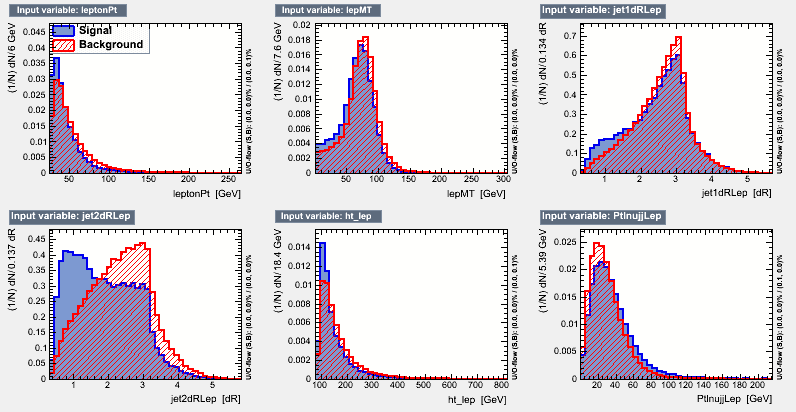
\includegraphics[width=\textwidth]{\figpath/Chapter5/BDT_Performance_Plots/BDT_InputVars_2j0B_p1.png}
        \caption{}
        \label{fig:BDT_InputVars_2j0B_p1}
    \end{subfigure}

    \begin{subfigure}[t]{0.95\textwidth}
        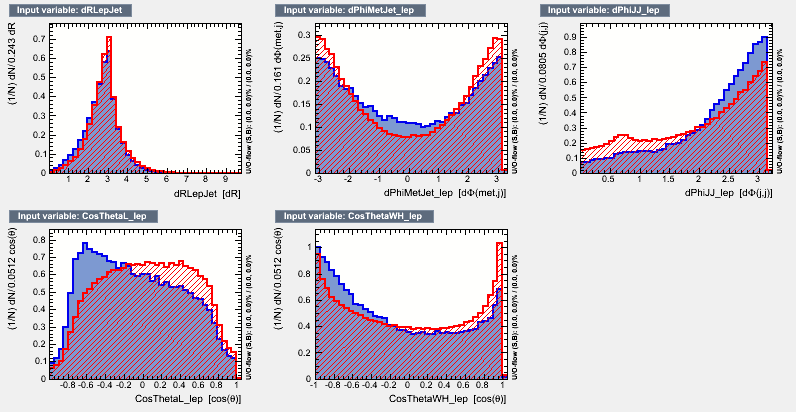
\includegraphics[width=\textwidth]{\figpath/Chapter5/BDT_Performance_Plots/BDT_InputVars_2j0B_p2.png}
        \caption{}
        \label{fig:BDT_InputVars_2j0B_p2}
    \end{subfigure}
    \caption{Inputs used to train the BDTs with kinematic variables in the 2 jets bin.}
    \label{fig:BDT_InputVars_2j0B}
\end{figure}

\begin{figure}[!hbt]
    \centering
    \begin{subfigure}[t]{0.95\textwidth}
        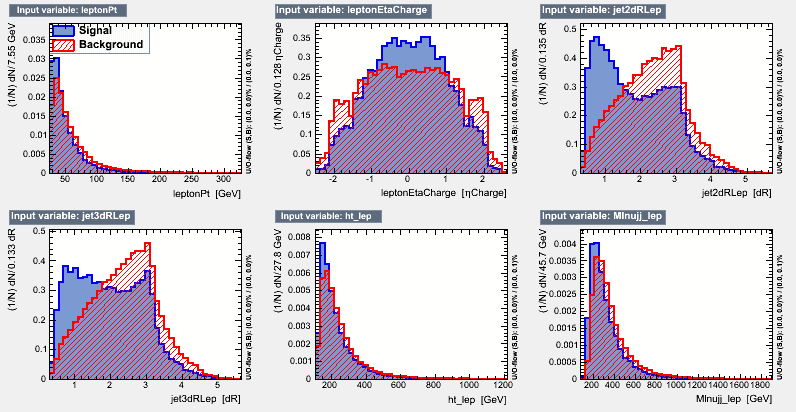
\includegraphics[width=\textwidth]{\figpath/Chapter5/BDT_Performance_Plots/BDT_InputVars_3j0B_p1.png}
        \caption{}
        \label{fig:BDT_InputVars_3j0B_p1}
    \end{subfigure}

    \begin{subfigure}[t]{0.95\textwidth}
        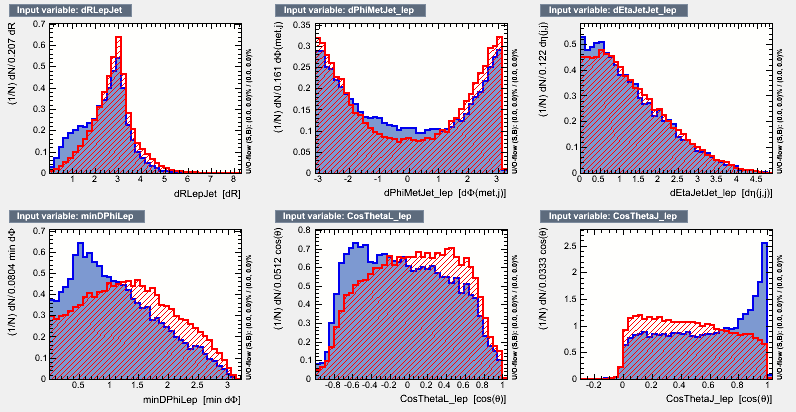
\includegraphics[width=\textwidth]{\figpath/Chapter5/BDT_Performance_Plots/BDT_InputVars_3j0B_p2.png}
        \caption{}
        \label{fig:BDT_InputVars_3j0B_p2}
    \end{subfigure}

    \begin{subfigure}[t]{0.95\textwidth}
        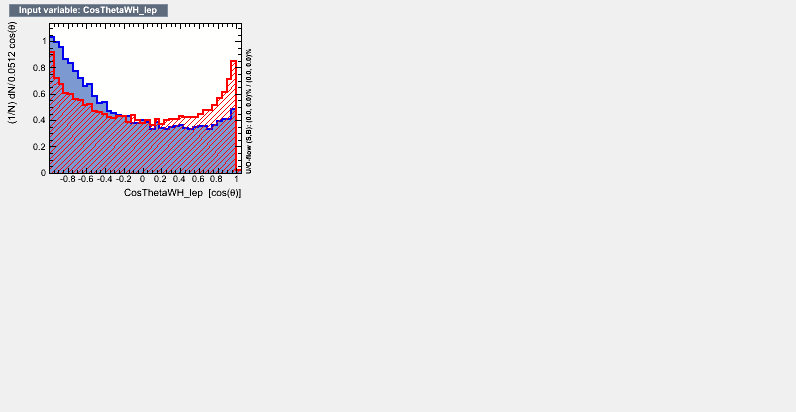
\includegraphics[trim={0 7.3cm 0 0},clip,width=\textwidth]{\figpath/Chapter5/BDT_Performance_Plots/BDT_InputVars_3j0B_p3.png}
        \caption{}
        \label{fig:BDT_InputVars_3j0B_p3}
    \end{subfigure}
    \caption{Inputs used to train the BDTs with kinematic variables in the 3 jets bin.}
    \label{fig:BDT_InputVars_3j0B}
\end{figure}

\begin{figure}[!hbt]
    \centering
    \begin{subfigure}[t]{0.95\textwidth}
        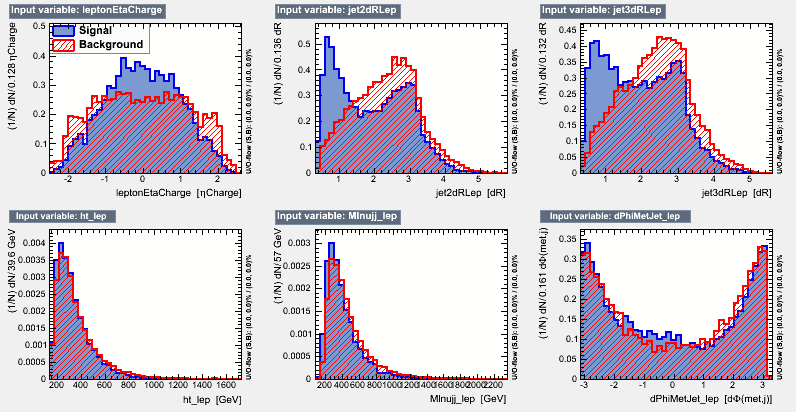
\includegraphics[width=\textwidth]{\figpath/Chapter5/BDT_Performance_Plots/BDT_InputVars_4j0B_p1.png}
        \caption{}
        \label{fig:BDT_InputVars_4j0B_p1}
    \end{subfigure}

    \begin{subfigure}[t]{0.95\textwidth}
        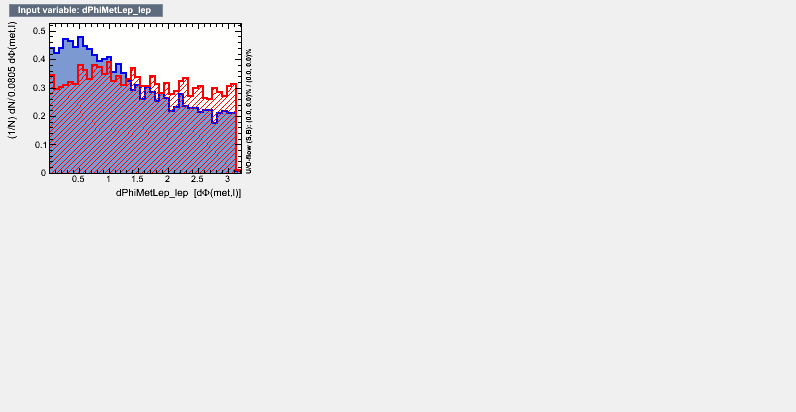
\includegraphics[width=\textwidth]{\figpath/Chapter5/BDT_Performance_Plots/BDT_InputVars_4j0B_p2.png}
        \caption{}
        \label{fig:BDT_InputVars_4j0B_p2}
    \end{subfigure}
    \caption{Inputs used to train the BDTs with kinematic variables in the $\geqslant$4 jets bin.}
    \label{fig:BDT_InputVars_4j0B}
\end{figure}
\clearpage
















\section{Outputs}
\label{appendix:BDT_Outputs}
\begin{figure}[!hbt]
    \centering
    \begin{subfigure}[t]{0.317\textwidth}
        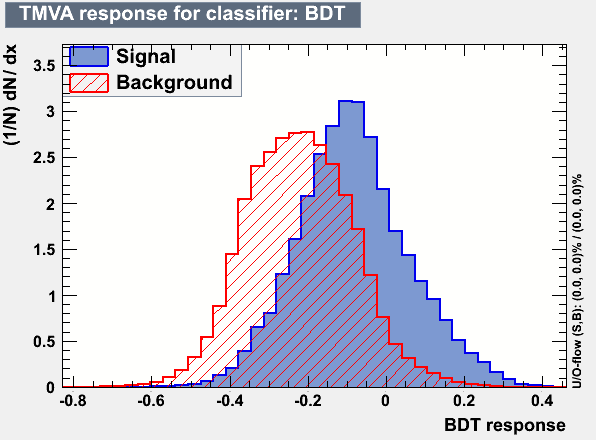
\includegraphics[width=\textwidth]{\figpath/Chapter5/BDT_Performance_Plots/BDT_Response_2j0B.png}
        \caption{}
        \label{fig:BDT_Response_2j0B_TMVA}
    \end{subfigure}
    \begin{subfigure}[t]{0.317\textwidth}
        \includegraphics[width=\textwidth]{\figpath/Appendix5/jets2/electron/KinBDT_electron.eps}
        \caption{}
        \label{fig:KinBDT_jets2_electron_noSys}
    \end{subfigure}
    \begin{subfigure}[t]{0.317\textwidth}
        \includegraphics[width=\textwidth]{\figpath/Appendix5/jets2/muon/KinBDT_muon.eps}
        \caption{}
        \label{fig:KinBDT_jets2_muon_noSys}
    \end{subfigure}
    \caption{(a) The BDT response plot from TMVA for the training with only kinematic variables in the 2 jet bin for the combined lepton channel. Validation plot for the BDT in the 2 jet bin for the (b) electron and (c) muon channels. Only statistical uncertainties are shown in the validation plots.}
    \label{fig:KinBDT_Comparison_jets2}
\end{figure}

\begin{figure}[!hbt]
    \centering
    \begin{subfigure}[t]{0.317\textwidth}
        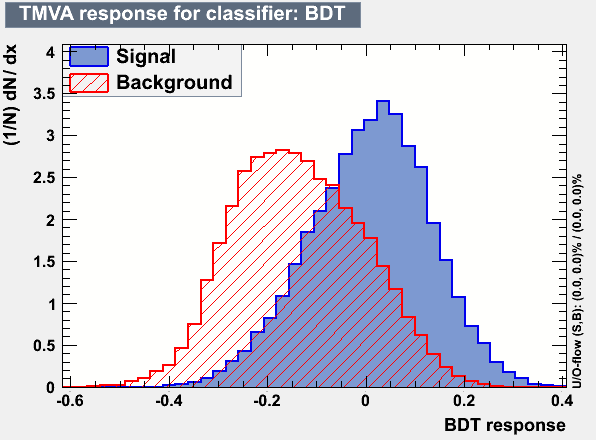
\includegraphics[width=\textwidth]{\figpath/Chapter5/BDT_Performance_Plots/BDT_Response_3j0B.png}
        \caption{}
        \label{fig:BDT_Response_3j0B_TMVA}
    \end{subfigure}
    \begin{subfigure}[t]{0.317\textwidth}
        \includegraphics[width=\textwidth]{\figpath/Appendix5/jets3/electron/KinBDT_electron.eps}
        \caption{}
        \label{fig:KinBDT_jets3_electron_noSys}
    \end{subfigure}
    \begin{subfigure}[t]{0.317\textwidth}
        \includegraphics[width=\textwidth]{\figpath/Appendix5/jets3/muon/KinBDT_muon.eps}
        \caption{}
        \label{fig:KinBDT_jets3_muon_noSys}
    \end{subfigure}
    \caption{(a) The BDT response plot from TMVA for the training with only kinematic variables in the 3 jet bin for the combined lepton channel. Validation plot for the BDT in the 3 jet bin for the (b) electron and (c) muon channels. Only statistical uncertainties are shown in the validation plots.}
    \label{fig:KinBDT_Comparison_jets3}
\end{figure}

\begin{figure}[!hbt]
    \centering
    \begin{subfigure}[t]{0.317\textwidth}
        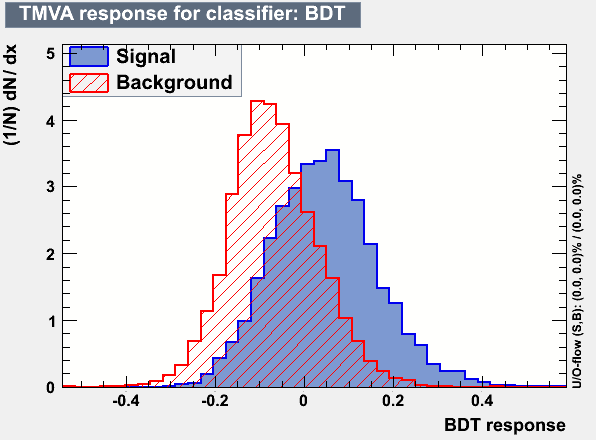
\includegraphics[width=\textwidth]{\figpath/Chapter5/BDT_Performance_Plots/BDT_Response_4j0B.png}
        \caption{}
        \label{fig:BDT_Response_4j0B_TMVA}
    \end{subfigure}
    \begin{subfigure}[t]{0.317\textwidth}
        \includegraphics[width=\textwidth]{\figpath/Appendix5/jets4/electron/KinBDT_electron.eps}
        \caption{}
        \label{fig:KinBDT_jets4_electron_noSys}
    \end{subfigure}
    \begin{subfigure}[t]{0.317\textwidth}
        \includegraphics[width=\textwidth]{\figpath/Appendix5/jets4/muon/KinBDT_muon.eps}
        \caption{}
        \label{fig:KinBDT_jets4_muon_noSys}
    \end{subfigure}
    \caption{(a) The BDT response plot from TMVA for the training with only kinematic variables in the $\geqslant$4 jet bin for the combined lepton channel. Validation plot for the BDT in the $\geqslant$4 jet bin for the (b) electron and (c) muon channels. Only statistical uncertainties are shown in the validation plots.}
    \label{fig:KinBDT_Comparison_jets4}
\end{figure}

\begin{figure}[!hbt]
    \centering
    \begin{subfigure}[t]{0.317\textwidth}
        \includegraphics[width=\textwidth]{\figpath/Appendix5/jets2/2015_07_17_TMVA_output_jets2_eq0tag_both_HToWW_WJets_allEvtProbs_0KinVar/mva_BDT.pdf}
        \caption{}
        \label{fig:MEBDT_Response_2j0B_TMVA}
    \end{subfigure}
    \begin{subfigure}[t]{0.317\textwidth}
        \includegraphics[width=\textwidth]{\figpath/Appendix5/jets2/electron/MEBDT_electron.eps}
        \caption{}
        \label{fig:MEBDT_jets2_electron_noSys}
    \end{subfigure}
    \begin{subfigure}[t]{0.317\textwidth}
        \includegraphics[width=\textwidth]{\figpath/Appendix5/jets2/muon/MEBDT_muon.eps}
        \caption{}
        \label{fig:MEBDT_jets2_muon_noSys}
    \end{subfigure}
    \caption{(a) The BDT response plot from TMVA for the training with only matrix element probabilities in the 2 jet bin for the combined lepton channel. Validation plot for the BDT in the 2 jet bin for the (b) electron and (c) muon channels. Only statistical uncertainties are shown in the validation plots.}
    \label{fig:MEBDT_Comparison_jets2}
\end{figure}

\begin{figure}[!hbt]
    \centering
    \begin{subfigure}[t]{0.317\textwidth}
        \includegraphics[width=\textwidth]{\figpath/Appendix5/jets3/2015_07_17_TMVA_output_jets3_eq0tag_both_HToWW_WJets_allEvtProbs_0KinVar/mva_BDT.pdf}
        \caption{}
        \label{fig:MEBDT_Response_3j0B_TMVA}
    \end{subfigure}
    \begin{subfigure}[t]{0.317\textwidth}
        \includegraphics[width=\textwidth]{\figpath/Appendix5/jets3/electron/MEBDT_electron.eps}
        \caption{}
        \label{fig:MEBDT_jets3_electron_noSys}
    \end{subfigure}
    \begin{subfigure}[t]{0.317\textwidth}
        \includegraphics[width=\textwidth]{\figpath/Appendix5/jets3/muon/MEBDT_muon.eps}
        \caption{}
        \label{fig:MEBDT_jets3_muon_noSys}
    \end{subfigure}
    \caption{(a) The BDT response plot from TMVA for the training with only matrix element probabilities in the 3 jet bin for the combined lepton channel. Validation plot for the BDT in the 3 jet bin for the (b) electron and (c) muon channels. Only statistical uncertainties are shown in the validation plots.}
    \label{fig:MEBDT_Comparison_jets3}
\end{figure}

\begin{figure}[!hbt]
    \centering
    \begin{subfigure}[t]{0.317\textwidth}
        \includegraphics[width=\textwidth]{\figpath/Appendix5/jets4/2015_07_17_TMVA_output_jets4_eq0tag_both_HToWW_WJets_allEvtProbs_0KinVar/mva_BDT.pdf}
        \caption{}
        \label{fig:MEBDT_Response_4j0B_TMVA}
    \end{subfigure}
    \begin{subfigure}[t]{0.317\textwidth}
        \includegraphics[width=\textwidth]{\figpath/Appendix5/jets4/electron/MEBDT_electron.eps}
        \caption{}
        \label{fig:MEBDT_jets4_electron_noSys}
    \end{subfigure}
    \begin{subfigure}[t]{0.317\textwidth}
        \includegraphics[width=\textwidth]{\figpath/Appendix5/jets4/muon/MEBDT_muon.eps}
        \caption{}
        \label{fig:MEBDT_jets4_muon_noSys}
    \end{subfigure}
    \caption{(a) The BDT response plot from TMVA for the training with only matrix element probabilities in the $\geqslant$4 jet bin for the combined lepton channel. Validation plot for the BDT in the $\geqslant$4 jet bin for the (b) electron and (c) muon channels. Only statistical uncertainties are shown in the validation plots.}
    \label{fig:MEBDT_Comparison_jets4}
\end{figure}

\begin{figure}[!hbt]
    \centering
    \begin{subfigure}[t]{0.317\textwidth}
        \includegraphics[width=\textwidth]{\figpath/Appendix5/jets2/2015_07_17_TMVA_output_jets2_eq0tag_both_HToWW_WJets_noEvtProbs_12KinVar/mva_BDT.pdf}
        \caption{}
        \label{fig:KinMEBDT_Response_2j0B_TMVA}
    \end{subfigure}
    \begin{subfigure}[t]{0.317\textwidth}
        \includegraphics[width=\textwidth]{\figpath/Appendix5/jets2/electron/KinMEBDT_electron.eps}
        \caption{}
        \label{fig:KinMEBDT_jets2_electron_noSys}
    \end{subfigure}
    \begin{subfigure}[t]{0.317\textwidth}
        \includegraphics[width=\textwidth]{\figpath/Appendix5/jets2/muon/KinMEBDT_muon.eps}
        \caption{}
        \label{fig:KinMEBDT_jets2_muon_noSys}
    \end{subfigure}
    \caption{(a) The BDT response plot from TMVA for the training with the kinematic variables and the ME BDT in the 2 jet bin for the combined lepton channel. Validation plot for the BDT in the 2 jet bin for the (b) electron and (c) muon channels. Only statistical uncertainties are shown in the validation plots.}
    \label{fig:KinMEBDT_Comparison_jets2}
\end{figure}

\begin{figure}[!hbt]
    \centering
    \begin{subfigure}[t]{0.317\textwidth}
        \includegraphics[width=\textwidth]{\figpath/Appendix5/jets3/2015_07_17_TMVA_output_jets3_eq0tag_both_HToWW_WJets_noEvtProbs_14KinVar/mva_BDT.pdf}
        \caption{}
        \label{fig:KinMEBDT_Response_3j0B_TMVA}
    \end{subfigure}
    \begin{subfigure}[t]{0.317\textwidth}
        \includegraphics[width=\textwidth]{\figpath/Appendix5/jets3/electron/KinMEBDT_electron.eps}
        \caption{}
        \label{fig:KinMEBDT_jets3_electron_noSys}
    \end{subfigure}
    \begin{subfigure}[t]{0.317\textwidth}
        \includegraphics[width=\textwidth]{\figpath/Appendix5/jets3/muon/KinMEBDT_muon.eps}
        \caption{}
        \label{fig:KinMEBDT_jets3_muon_noSys}
    \end{subfigure}
    \caption{(a) The BDT response plot from TMVA for the training with the kinematic variables and the ME BDT in the 3 jet bin for the combined lepton channel. Validation plot for the BDT in the 3 jet bin for the (b) electron and (c) muon channels. Only statistical uncertainties are shown in the validation plots.}
    \label{fig:KinMEBDT_Comparison_jets3}
\end{figure}

\begin{figure}[!hbt]
    \centering
    \begin{subfigure}[t]{0.317\textwidth}
        \includegraphics[width=\textwidth]{\figpath/Appendix5/jets4/2015_07_17_TMVA_output_jets4_eq0tag_both_HToWW_WJets_noEvtProbs_8KinVar/mva_BDT.pdf}
        \caption{}
        \label{fig:KinMEBDT_Response_4j0B_TMVA}
    \end{subfigure}
    \begin{subfigure}[t]{0.317\textwidth}
        \includegraphics[width=\textwidth]{\figpath/Appendix5/jets4/electron/KinMEBDT_electron.eps}
        \caption{}
        \label{fig:KinMEBDT_jets4_electron_noSys}
    \end{subfigure}
    \begin{subfigure}[t]{0.317\textwidth}
        \includegraphics[width=\textwidth]{\figpath/Appendix5/jets4/muon/KinMEBDT_muon.eps}
        \caption{}
        \label{fig:KinMEBDT_jets4_muon_noSys}
    \end{subfigure}
    \caption{(a) The BDT response plot from TMVA for the training with the kinematic variables and the ME BDT in the $\geqslant$4 jet bin for the combined lepton channel. Validation plot for the BDT in the $\geqslant$4 jet bin for the (b) electron and (c) muon channels. Only statistical uncertainties are shown in the validation plots.}
    \label{fig:KinMEBDT_Comparison_jets4}
\end{figure}
\clearpage







\section{Correlations}
\label{appendix:BDT_Correlations}

\begin{figure}[!hbt]
    \centering
    \begin{subfigure}[t]{0.48\textwidth}
        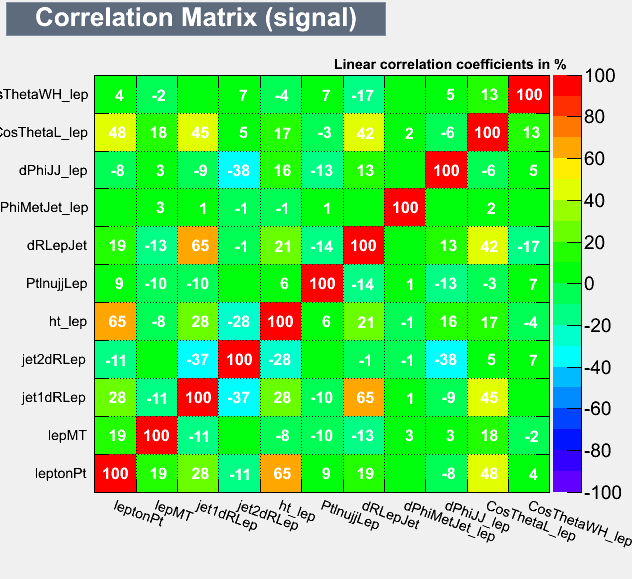
\includegraphics[width=\textwidth]{\figpath/Chapter5/BDT_Performance_Plots/CorrelationMatrixS_2j0B.png}
        \caption{}
        \label{fig:KinBDT_jets2_CorrelationS}
    \end{subfigure}
    \begin{subfigure}[t]{0.48\textwidth}
        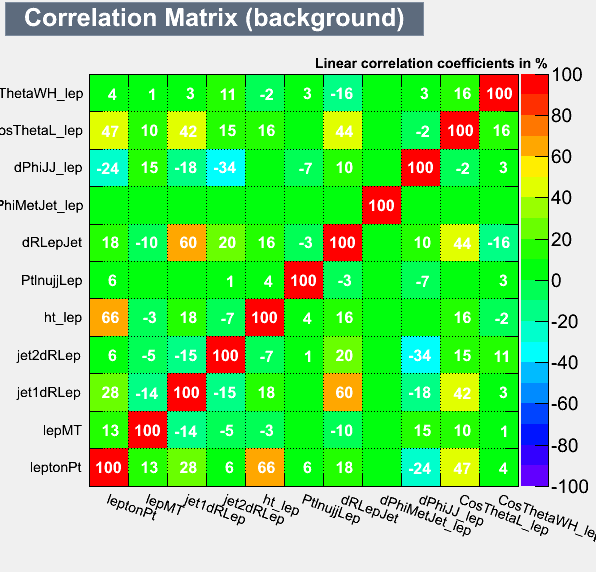
\includegraphics[width=\textwidth]{\figpath/Chapter5/BDT_Performance_Plots/CorrelationMatrixB_2j0B.png}
        \caption{}
        \label{fig:KinBDT_jets2_CorrelationB}
    \end{subfigure}
    \caption{Correlation plots for (a) signal and (b) background for the BDT trained with only kinematic variables in the 2 jet bin.}
    \label{fig:KinBDT_jets2_Correlations}
\end{figure}

\begin{figure}[!hbt]
    \centering
    \begin{subfigure}[t]{0.48\textwidth}
        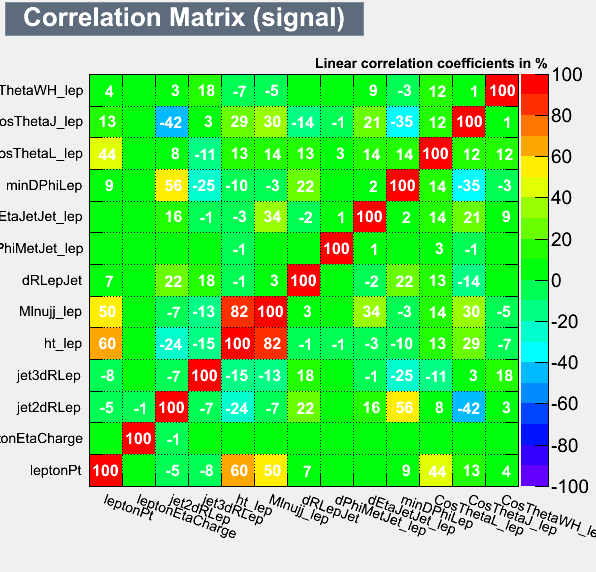
\includegraphics[width=\textwidth]{\figpath/Chapter5/BDT_Performance_Plots/CorrelationMatrixS_3j0B.png}
        \caption{}
        \label{fig:KinBDT_jets3_CorrelationS}
    \end{subfigure}
    \begin{subfigure}[t]{0.48\textwidth}
        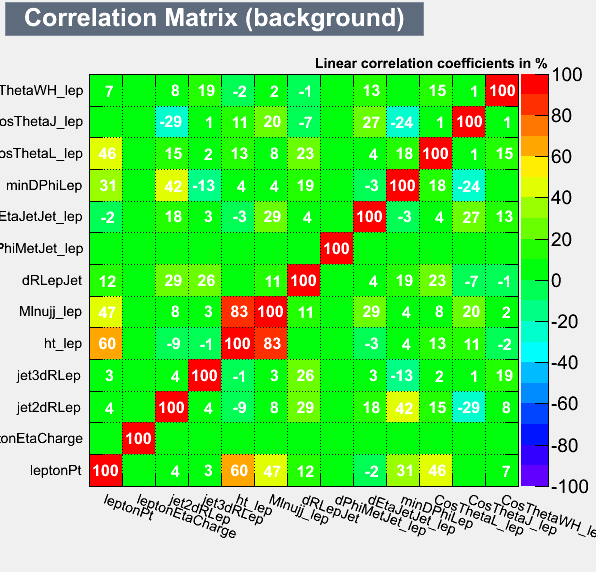
\includegraphics[width=\textwidth]{\figpath/Chapter5/BDT_Performance_Plots/CorrelationMatrixB_3j0B.png}
        \caption{}
        \label{fig:KinBDT_jets3_CorrelationB}
    \end{subfigure}
    \caption{Correlation plots for (a) signal and (b) background for the BDT trained with only kinematic variables in the 3 jet bin.}
    \label{fig:KinBDT_jets3_Correlations}
\end{figure}

\begin{figure}[!hbt]
    \centering
    \begin{subfigure}[t]{0.48\textwidth}
        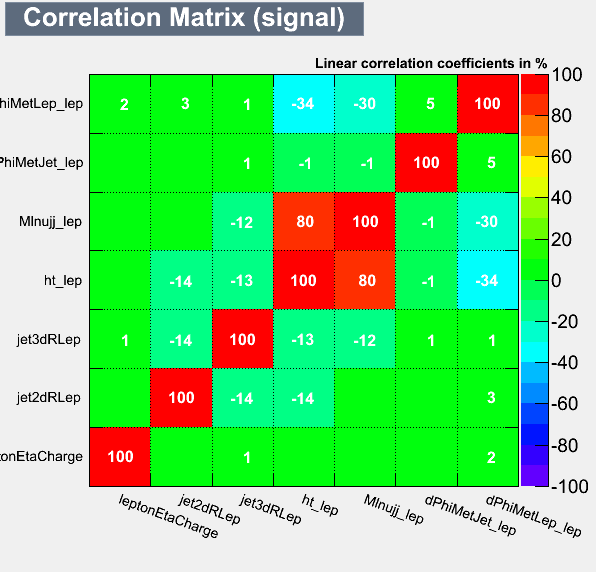
\includegraphics[width=\textwidth]{\figpath/Chapter5/BDT_Performance_Plots/CorrelationMatrixS_4j0B.png}
        \caption{}
        \label{fig:KinBDT_jets4_CorrelationS}
    \end{subfigure}
    \begin{subfigure}[t]{0.48\textwidth}
        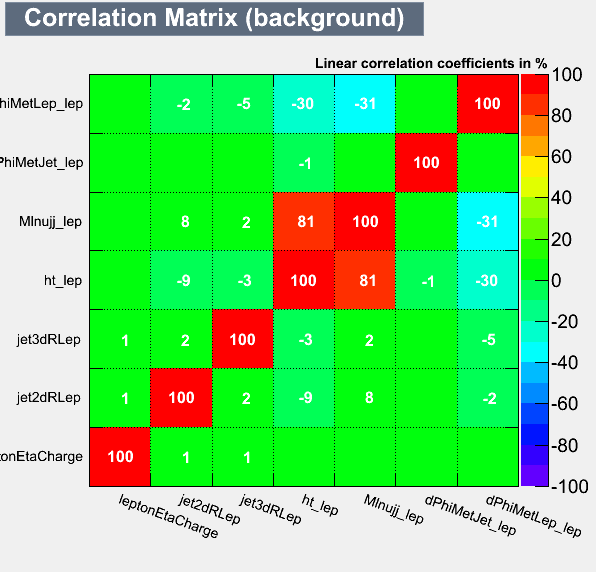
\includegraphics[width=\textwidth]{\figpath/Chapter5/BDT_Performance_Plots/CorrelationMatrixB_4j0B.png}
        \caption{}
        \label{fig:KinBDT_jets4_CorrelationB}
    \end{subfigure}
    \caption{Correlation plots for (a) signal and (b) background for the BDT trained with only kinematic variables in the $\geqslant$4 jet bin.}
    \label{fig:KinBDT_jets4_Correlations}
\end{figure}

\begin{figure}[!hbt]
    \centering
    \begin{subfigure}[t]{0.48\textwidth}
        \includegraphics[width=\textwidth]{\figpath/Appendix5/jets2/2015_07_17_TMVA_output_jets2_eq0tag_both_HToWW_WJets_allEvtProbs_0KinVar/CorrelationMatrixS.pdf}
        \caption{}
        \label{fig:MEBDT_jets2_CorrelationS}
    \end{subfigure}
    \begin{subfigure}[t]{0.48\textwidth}
        \includegraphics[width=\textwidth]{\figpath/Appendix5/jets2/2015_07_17_TMVA_output_jets2_eq0tag_both_HToWW_WJets_allEvtProbs_0KinVar/CorrelationMatrixB.pdf}
        \caption{}
        \label{fig:MEBDT_jets2_CorrelationB}
    \end{subfigure}
    \caption{Correlation plots for (a) signal and (b) background for the BDT trained with only matrix elements variables in the 2 jet bin.}
    \label{fig:MEBDT_jets2_Correlations}
\end{figure}

\begin{figure}[!hbt]
    \centering
    \begin{subfigure}[t]{0.48\textwidth}
        \includegraphics[width=\textwidth]{\figpath/Appendix5/jets3/2015_07_17_TMVA_output_jets3_eq0tag_both_HToWW_WJets_allEvtProbs_0KinVar/CorrelationMatrixS.pdf}
        \caption{}
        \label{fig:MEBDT_jets3_CorrelationS}
    \end{subfigure}
    \begin{subfigure}[t]{0.48\textwidth}
        \includegraphics[width=\textwidth]{\figpath/Appendix5/jets3/2015_07_17_TMVA_output_jets3_eq0tag_both_HToWW_WJets_allEvtProbs_0KinVar/CorrelationMatrixB.pdf}
        \caption{}
        \label{fig:MEBDT_jets3_CorrelationB}
    \end{subfigure}
    \caption{Correlation plots for (a) signal and (b) background for the BDT trained with only matrix elements variables in the 3 jet bin.}
    \label{fig:MEBDT_jets3_Correlations}
\end{figure}

\begin{figure}[!hbt]
    \centering
    \begin{subfigure}[t]{0.48\textwidth}
        \includegraphics[width=\textwidth]{\figpath/Appendix5/jets4/2015_07_17_TMVA_output_jets4_eq0tag_both_HToWW_WJets_allEvtProbs_0KinVar/CorrelationMatrixS.pdf}
        \caption{}
        \label{fig:MEBDT_jets4_CorrelationS}
    \end{subfigure}
    \begin{subfigure}[t]{0.48\textwidth}
        \includegraphics[width=\textwidth]{\figpath/Appendix5/jets4/2015_07_17_TMVA_output_jets4_eq0tag_both_HToWW_WJets_allEvtProbs_0KinVar/CorrelationMatrixB.pdf}
        \caption{}
        \label{fig:MEBDT_jets4_CorrelationB}
    \end{subfigure}
    \caption{Correlation plots for (a) signal and (b) background for the BDT trained with only matrix elements variables in the $\geqslant$4 jet bin.}
    \label{fig:MEBDT_jets4_Correlations}
\end{figure}

\begin{figure}[!hbt]
    \centering
    \begin{subfigure}[t]{0.48\textwidth}
        \includegraphics[width=\textwidth]{\figpath/Appendix5/jets2/2015_07_17_TMVA_output_jets2_eq0tag_both_HToWW_WJets_noEvtProbs_12KinVar/CorrelationMatrixS.pdf}
        \caption{}
        \label{fig:KinMEBDT_jets2_CorrelationS}
    \end{subfigure}
    \begin{subfigure}[t]{0.48\textwidth}
        \includegraphics[width=\textwidth]{\figpath/Appendix5/jets2/2015_07_17_TMVA_output_jets2_eq0tag_both_HToWW_WJets_noEvtProbs_12KinVar/CorrelationMatrixB.pdf}
        \caption{}
        \label{fig:KinMEBDT_jets2_CorrelationB}
    \end{subfigure}
    \caption{Correlation plots for (a) signal and (b) background for the BDT trained with both the kinematic variables and the ME BDT in the 2 jet bin.}
    \label{fig:KinMEBDT_jets2_Correlations}
\end{figure}

\begin{figure}[!hbt]
    \centering
    \begin{subfigure}[t]{0.48\textwidth}
        \includegraphics[width=\textwidth]{\figpath/Appendix5/jets3/2015_07_17_TMVA_output_jets3_eq0tag_both_HToWW_WJets_noEvtProbs_14KinVar/CorrelationMatrixS.pdf}
        \caption{}
        \label{fig:KinMEBDT_jets3_CorrelationS}
    \end{subfigure}
    \begin{subfigure}[t]{0.48\textwidth}
        \includegraphics[width=\textwidth]{\figpath/Appendix5/jets3/2015_07_17_TMVA_output_jets3_eq0tag_both_HToWW_WJets_noEvtProbs_14KinVar/CorrelationMatrixB.pdf}
        \caption{}
        \label{fig:KinMEBDT_jets3_CorrelationB}
    \end{subfigure}
    \caption{Correlation plots for (a) signal and (b) background for the BDT trained with both the kinematic variables and the ME BDT in the 3 jet bin.}
    \label{fig:KinMEBDT_jets3_Correlations}
\end{figure}

\begin{figure}[!hbt]
    \centering
    \begin{subfigure}[t]{0.48\textwidth}
        \includegraphics[width=\textwidth]{\figpath/Appendix5/jets4/2015_07_17_TMVA_output_jets4_eq0tag_both_HToWW_WJets_noEvtProbs_8KinVar/CorrelationMatrixS.pdf}
        \caption{}
        \label{fig:KinMEBDT_jets4_CorrelationS}
    \end{subfigure}
    \begin{subfigure}[t]{0.48\textwidth}
        \includegraphics[width=\textwidth]{\figpath/Appendix5/jets4/2015_07_17_TMVA_output_jets4_eq0tag_both_HToWW_WJets_noEvtProbs_8KinVar/CorrelationMatrixB.pdf}
        \caption{}
        \label{fig:KinMEBDT_jets4_CorrelationB}
    \end{subfigure}
    \caption{Correlation plots for (a) signal and (b) background for the BDT trained with both the kinematic variables and the ME BDT in the $\geqslant$4 jet bin.}
    \label{fig:KinMEBDT_jets4_Correlations}
\end{figure}
\clearpage







\section{ROC Curves}
\label{appendix:BDT_ROC_curves}
\begin{figure}[!hbt]
    \centering
    \begin{subfigure}[t]{0.316\textwidth}
        \includegraphics[width=\textwidth]{\figpath/Appendix5/jets2/2015_07_17_TMVA_output_jets2_eq0tag_both_HToWW_WJets_noEvtProbs_11KinVar/rejBvsS_BDT_simple.pdf}
        \caption{}
        \label{fig:KinBDT_ROC_jets2}
    \end{subfigure}
    \begin{subfigure}[t]{0.316\textwidth}
        \includegraphics[width=\textwidth]{\figpath/Appendix5/jets3/2015_07_17_TMVA_output_jets3_eq0tag_both_HToWW_WJets_noEvtProbs_13KinVar/rejBvsS_BDT_simple.pdf}
        \caption{}
        \label{fig:KinBDT_ROC_jets3}
    \end{subfigure}
    \begin{subfigure}[t]{0.316\textwidth}
        \includegraphics[width=\textwidth]{\figpath/Appendix5/jets4/2015_07_17_TMVA_output_jets4_eq0tag_both_HToWW_WJets_noEvtProbs_7KinVar/rejBvsS_BDT_simple.pdf}
        \caption{}
        \label{fig:KinBDT_ROC_jets4}
    \end{subfigure}

    \begin{subfigure}[t]{0.316\textwidth}
        \includegraphics[width=\textwidth]{\figpath/Appendix5/jets2/2015_07_17_TMVA_output_jets2_eq0tag_both_HToWW_WJets_allEvtProbs_0KinVar/rejBvsS_BDT_simple.pdf}
        \caption{}
        \label{fig:MEBDT_ROC_jets2}
    \end{subfigure}
    \begin{subfigure}[t]{0.316\textwidth}
        \includegraphics[width=\textwidth]{\figpath/Appendix5/jets3/2015_07_17_TMVA_output_jets3_eq0tag_both_HToWW_WJets_allEvtProbs_0KinVar/rejBvsS_BDT_simple.pdf}
        \caption{}
        \label{fig:MEBDT_ROC_jets3}
    \end{subfigure}
    \begin{subfigure}[t]{0.316\textwidth}
        \includegraphics[width=\textwidth]{\figpath/Appendix5/jets4/2015_07_17_TMVA_output_jets4_eq0tag_both_HToWW_WJets_allEvtProbs_0KinVar/rejBvsS_BDT_simple.pdf}
        \caption{}
        \label{fig:MEBDT_ROC_jets4}
    \end{subfigure}

    \begin{subfigure}[t]{0.316\textwidth}
        \includegraphics[width=\textwidth]{\figpath/Appendix5/jets2/2015_07_17_TMVA_output_jets2_eq0tag_both_HToWW_WJets_noEvtProbs_12KinVar/rejBvsS_BDT_simple.pdf}
        \caption{}
        \label{fig:KinMEBDT_ROC_jets2}
    \end{subfigure}
    \begin{subfigure}[t]{0.316\textwidth}
        \includegraphics[width=\textwidth]{\figpath/Appendix5/jets3/2015_07_17_TMVA_output_jets3_eq0tag_both_HToWW_WJets_noEvtProbs_14KinVar/rejBvsS_BDT_simple.pdf}
        \caption{}
        \label{fig:KinMEBDT_ROC_jets3}
    \end{subfigure}
    \begin{subfigure}[t]{0.316\textwidth}
        \includegraphics[width=\textwidth]{\figpath/Appendix5/jets4/2015_07_17_TMVA_output_jets4_eq0tag_both_HToWW_WJets_noEvtProbs_8KinVar/rejBvsS_BDT_simple.pdf}
        \caption{}
        \label{fig:KinMEBDT_ROC_jets4}
    \end{subfigure}
    \caption{The receiver operating characteristic (ROC) curves for the various BDT trainings. The plots are ordered by jet bin from left to right, with the leftmost plot being the two-jet bin and the rightmost plot being the greater than or equal to four-jet bin. The top row contains the KinBDT plots while the middle and bottom rows contain the MEBDT and KinMEBDT plots, respectively.}
    \label{fig:BDT_ROC_all}
\end{figure}




\clearpage
